%---
\section{Introduction}\label{sec:intro}\label{sec:introduction}

\mymarginpar{keywords and PACS are from our papers - need updates?}

\dsf\ is a Liquid Argon Time Projection Chamber (\lar\ \tpc), operated in Italy's Gran Sasso National Laboratory (LNGS) to search for nuclear recoils induced by weakly interacting massive particles (WIMPs). The first physics result was reported in \cite{Agnes:2015gu} based on 50 live data collection days with Atmospheric Argon (AAr), providing the most sensitive limit on a dark matter search using a \lar\ \tpc\ to date with a 90\% CL upper limit on the WIMP-nucleon spin-independent cross section of $6.1 x 10^{-44}$ cm$^2$ for a WIMP mass of 100 GeV/c$^2$.  %along with two other key results: ar bg can be suppressed for ton-scale experiments using \uar and efficiency of the veto 

A first WIMP search using argon extracted from underground sources (Underground Argon, UAr) has been reported in \cite{Agnes:2015_uar}, following the WIMP search with AAr. UAr has a lower concentration of the radioactive $\beta$-emitter $^{39}$Ar by a factor (1.4 $\pm$ 0.2) $\times\, 10^3$ relative to AAr. Calibration campaigns have been performed in the presence of AAr and UAr.

The \dsf\ apparatus is described in detail in \cite{Agnes:2015gu}. As shown in fig.~\ref{fig:wholeAssembly_insideDetectors}, it features a \lar\ \tpc\ surrounded by a 30 t liquid scintillator-based veto (LSV) system, placed inside a water Cerenkov veto detector (\wcv), both of which measure in-situ and suppress radiogenic and cosmogenic backgrounds. On the top of the \wcv\ is a radon-free clean room (CRH) housing the cryogenic supply system and electronics (Fig.~\ref{fig:CALIS_photos}). The \lsv's inside is accessible from CRH through four access ports, called organ pipes, which are closed by gate valves. 

%After this introduction the CALIS design requirements and hardware realization are described in Sec.~\ref{sec:hardware}. Calibration campaigns and some of their physics highlights are discussed in Sec.~\ref{sec:CalibCampaigns}, before concluding in Sec.~\ref{sec:Conclusion}.

\begin{figure}[htbp]
 \centering
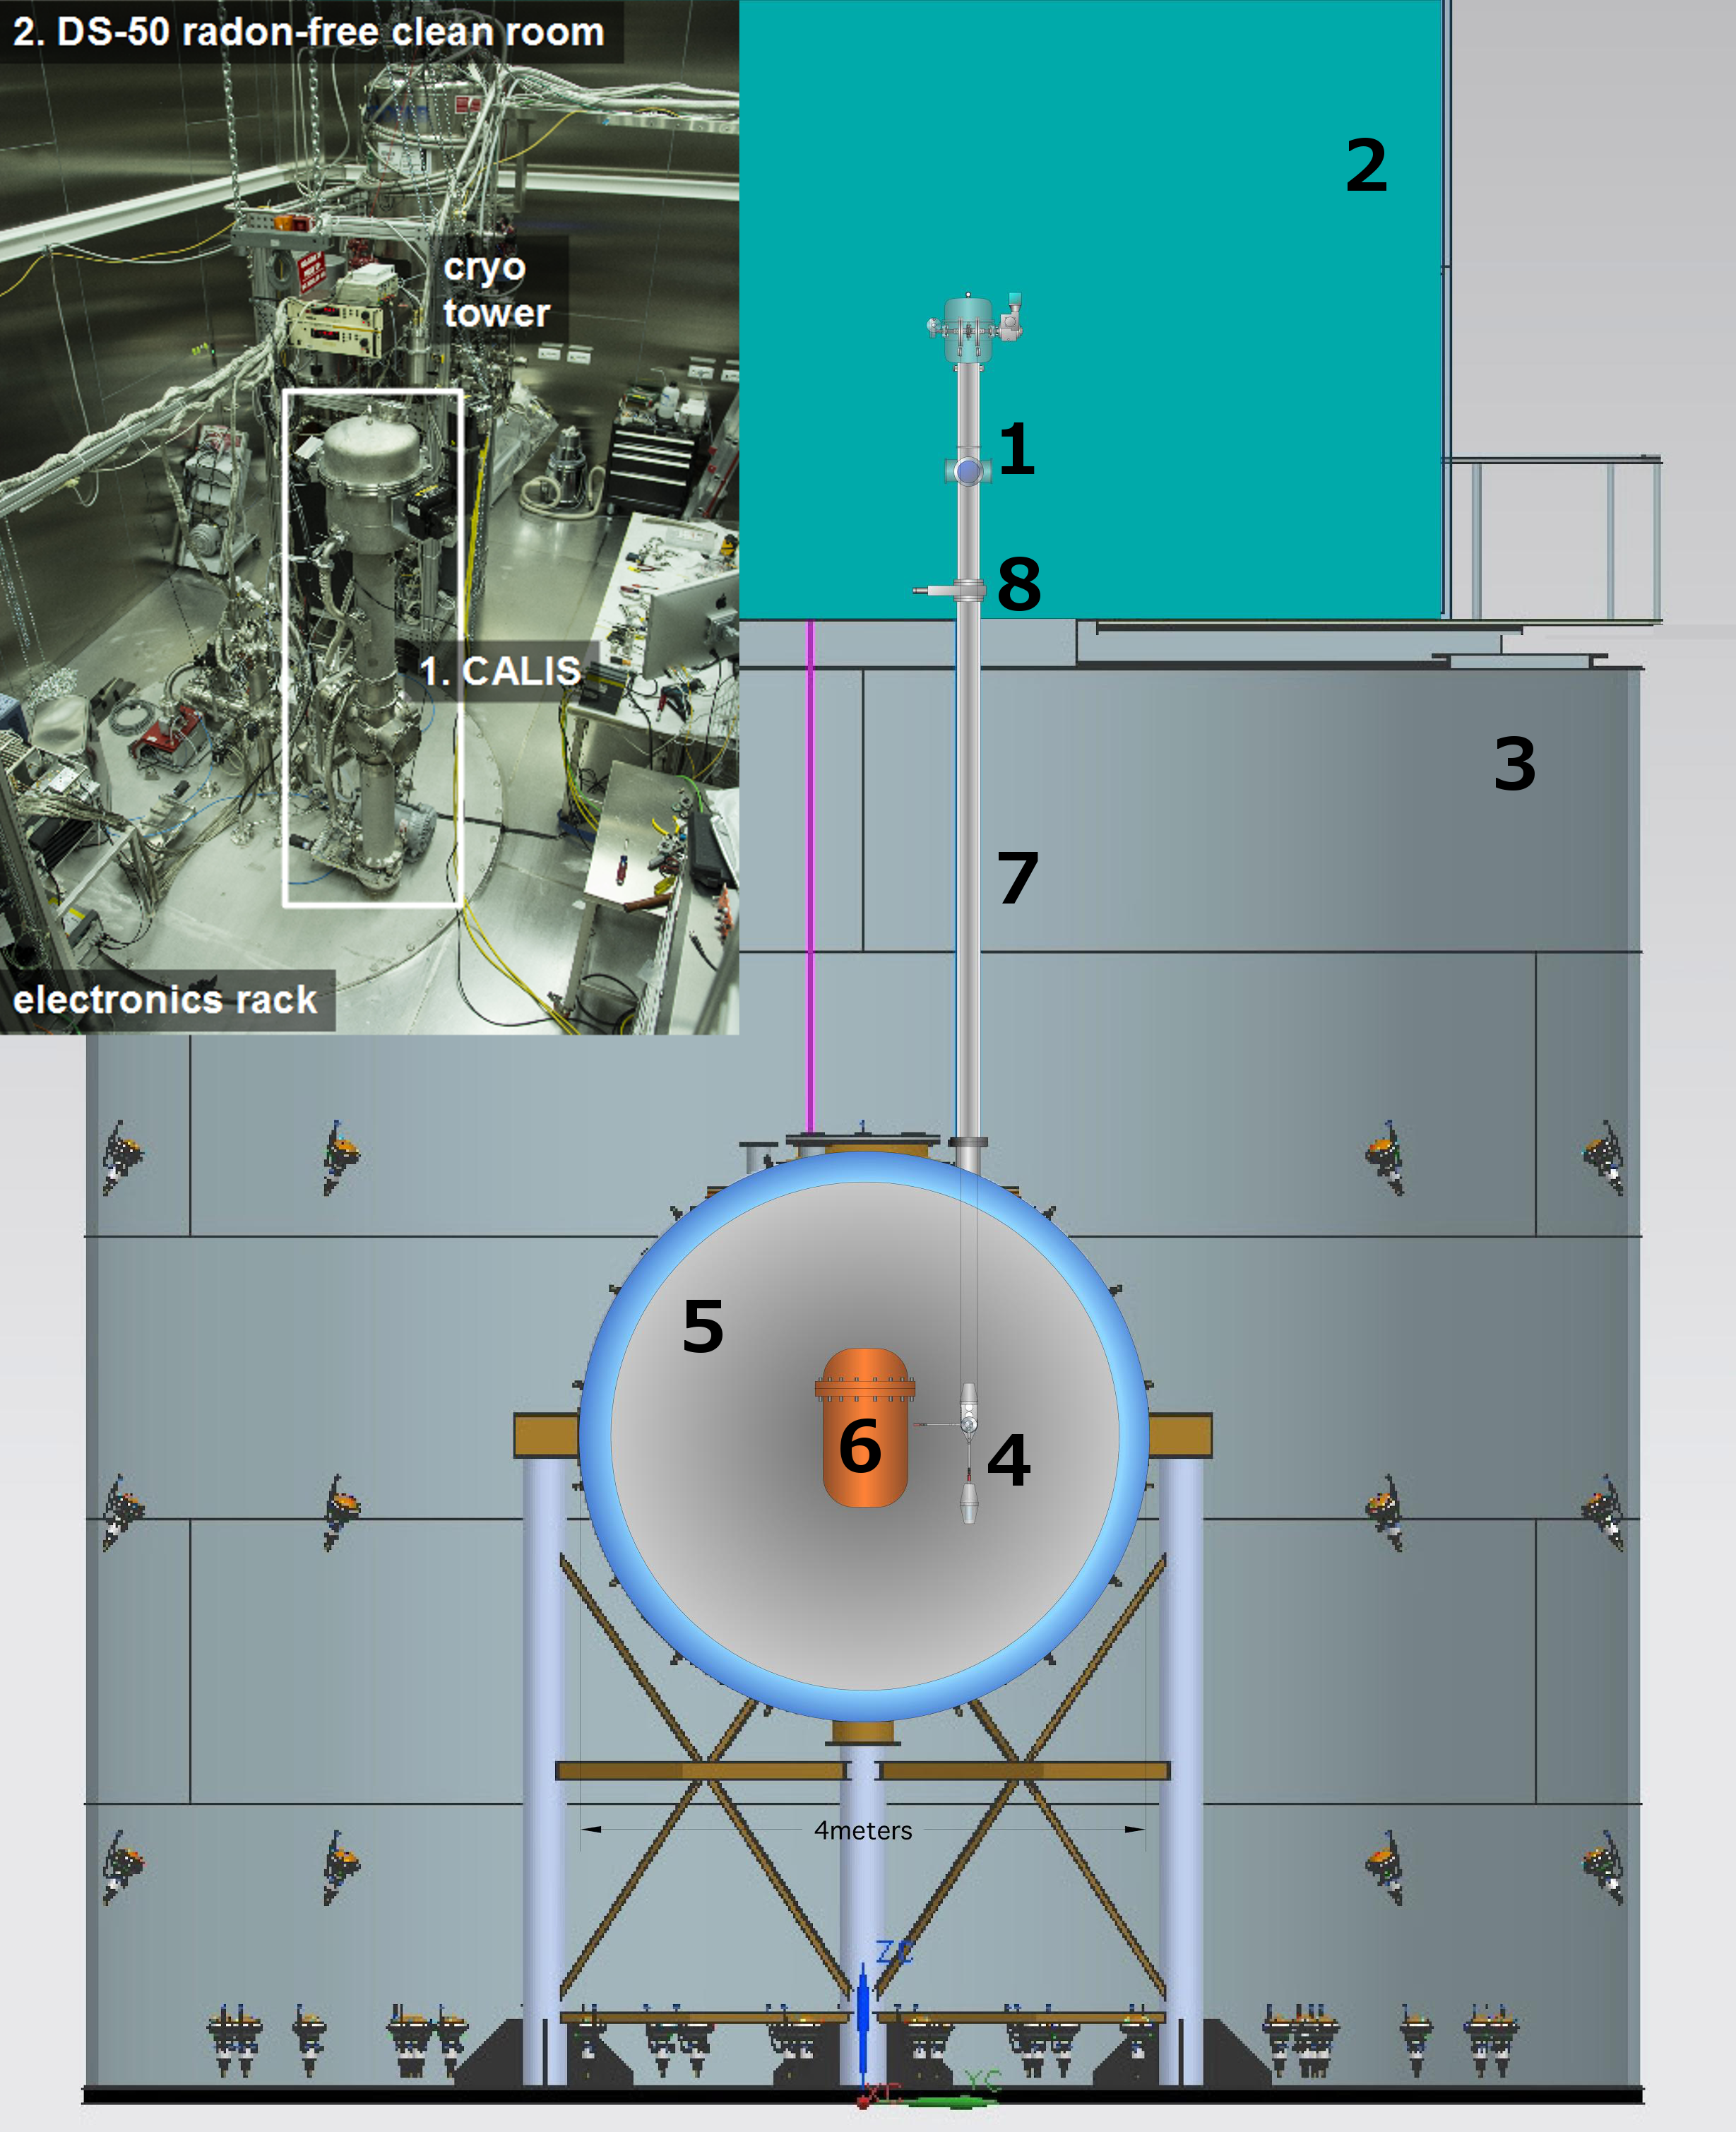
\includegraphics[width=0.95\textwidth]{Figures/DS50_with_CALIS}
\caption{A conceptual drawing of CALIS (1) installed in the radon-free clean room, CRH, (2) atop the water Cerenkov veto (\wcv, 3). The deployment device (4) which contains the source is deployed in the liquid scintillator veto (LSV, 5) next to the liquid argon time projection chamber's (\lar\ \tpc) cryostat (6). The clean room and the LSV are connected through four access ports, called organ pipes (only one of which is drawn in the above sketch (7)). All four organ pipes end in CRH at gate valves (8) which can be manually opened or closed. During normal operations all four organ pipes are closed. Not included in the sketch are tubes connecting the cryogenic systems in CRH to the cryostat in the \lsv\ \cite{Agnes:2015qyz}.\label{fig:wholeAssembly_insideDetectors}\label{fig:DS50_with_CALIS}}
\end{figure}

\begin{figure}[htbp]
 \centering
\subfigure{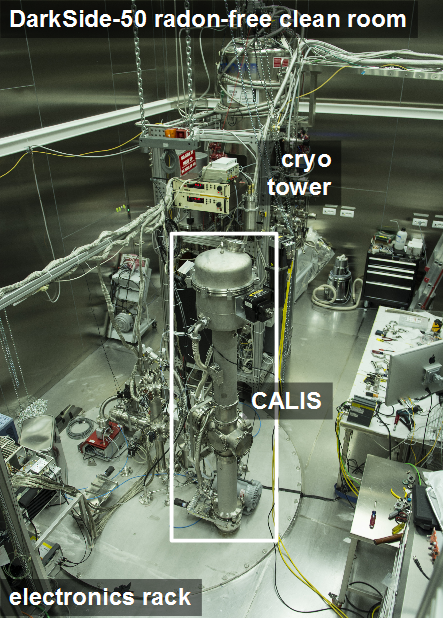
\includegraphics[width=0.335\textwidth]{./Figures/CALISinCRH_PetersComment.png}}
\subfigure{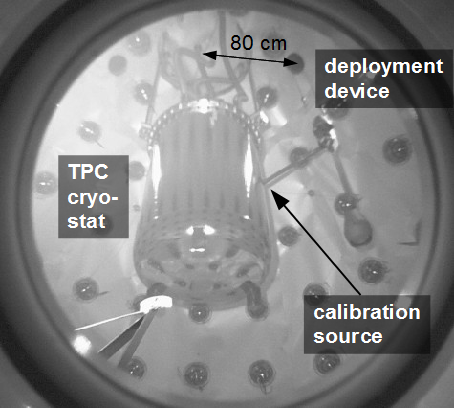
\includegraphics[width=0.52\textwidth]{./Figures/Next2Cryostat_80cm.png}}
\caption{\textit{Left}: CALIS after installation inside the radon-free clean room CRH. The organ pipe is 80 cm off-center with respect to the TPC's vertical Z-axis. \textit{Right}: Photograph taken with a camera looking upwards into the \lsv\ from the bottom. It shows the source deployment device deployed through one of the organ pipes visible on the top right. The arm is articulated and the source is next to the \lar\ \tpc's cryostat \cite{Agnes:2015qyz}.
\label{fig:CALIS_photos}}
\end{figure}


%time line plot, how did the veto change during the calibration campaigns - allowing for systematics studies.
%table on what was the goal of each campaign. What sources were used


%safety requirements

%design section
%installation: before, after

